\section{Evaluating WF+DNS Attacks}
\label{sec:analysis}

\subsection{Attack precision and recall}

To evaluate our WF+DNS attacks, we collected traffic traces in May
2016 using TBB~5.5.4.
We modified TBB so that it does not generate network traffic on launch
(\ie, check for
updates, extensions, etc.), and we modified 
Tor (bundled with TBB) to log incoming and outgoing cells.
We then collected performed 100 downloads for each site in the Alexa top
1k and one download for each site in the 
Alexa top (1k,101k]. We randomly distributed these measurement tasks
to a Docker fleet; each download used a fresh circuit without
guards and a fresh copy of TBB\footnote{The consensus was cached to not
cause an excessive load on the network.} for up to 60 seconds,
in line with the recommendations by Wang and Goldberg~\cite{Wang2013a}.
We considered the measurement to be successful if we managed to resolve
the domain of the site; 
we did not prune our dataset further, neglecting issues like CloudFlare
CAPTCHAs, outliers, control cells, and localized domains~\cite{Juarez2014a}.
This likely leads to overall worse results for all attacks than what is
possible, but we are primarily interested in the difference between WF and
WF+DNS attacks~\cite{Wang2013a}.

We perform ten-fold cross-validation for all of our experiments in the open
world setting, monitoring 1,000 sites with 100 instances each and
100,000 unmonitored sites unless otherwise stated.
Note the 1:1 ratio between monitored traces and unmonitored traces,
ensuring that for the classifier there is equal probability in the testing
phase that a trace is a monitored or unmonitored site.
In other words, the \emph{base rate} is 0.5 in our experiments.
Furthermore, for all experiments we specify the starting Alexa rank of the
monitored sites
\emph{when simulating sites visited over the Tor network}\footnote{We always
use the same sample data for website fingerprinting.}.
Whem minitoring 1000 sites starting at rank 1, sites
[1,1000] are monitored and Alexa [1001,101000] unmonitored. Starting to
monitor Alexa from rank 100 means that Alexa sites [101,1100] are monitored,
and Alexa [1,100] and [1101,10100] unmonitored.
We never monitor an unmonitored site or vice versa.
How popular monitored sites
are is a key factor in the effectiveness of our attacks.
% note: base rate is per user, while popularity in Alexa for DNS observations
% is world-wide

Figure~\ref{fig:wfdns:torpct} shows the recall and precision for our WF+DNS
attacks as a function of the percentage of observed Tor exit bandwidth by the
attacker monitoring Alexa sites from rank $10^5$.
For recall both \texttt{ctw} and \texttt{hp} are bound by the
percentage of exit bandwidth observed by the attacker (the percentage is an
upper bound).
Simply put, an attacker cannot identify a monitored site in the DNS data that
she does not see. Note that \texttt{ctw} sees improved recall over \texttt{wf}
at 100\% of exit bandwidth. For \texttt{hp} the results suggest that:
\begin{equation}
	\label{eq:hprecall}
	\textnormal{recall}_{\texttt{hp}} = \textnormal{recall}_{\texttt{wf}} * \textnormal{pct}
\end{equation}
Note that the above relationship only holds when observing DNS requests gives
a clear advantage to \texttt{hp} in terms of precision over \texttt{wf} (see
following paragraph).
For precision our attacks have an immediate gain over \texttt{wf} as soon as
the attacker can observe \emph{any exit bandwidth}.
While the \texttt{hp} attack has constantly near-perfect precision, the
\texttt{ctw} attack benefits from observing more and more of exit bandwidth,
nearly reaching the same levels as \texttt{hp} at 100\%.


\begin{figure}[t]
\centering
\subfigure[Recall]{
	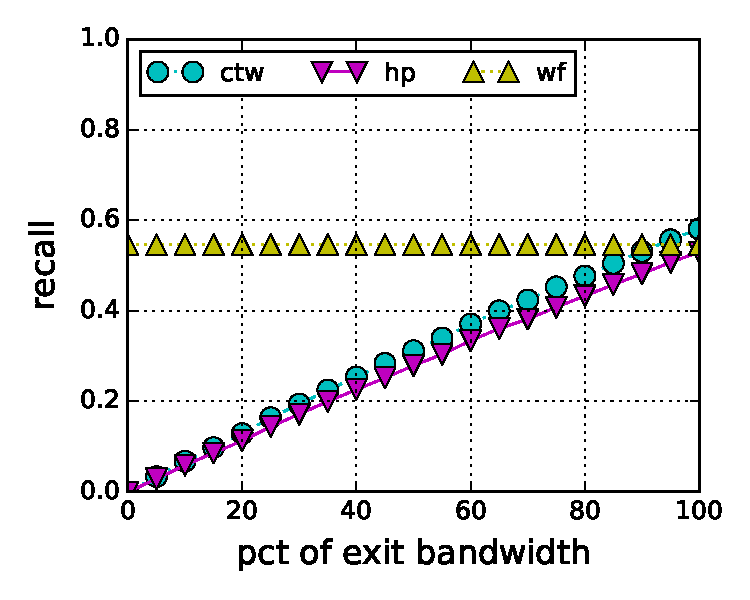
\includegraphics[width=0.466\linewidth]{figures/wfdns/pct/1kx100+100k-recall}
    \label{fig:wfdns:torpct:recall}
}
\subfigure[Precision]{
	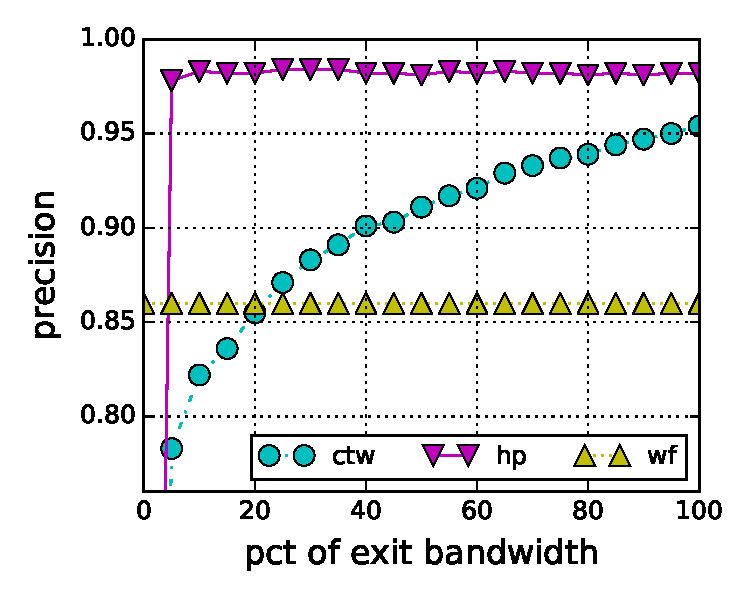
\includegraphics[width=0.466\linewidth]{figures/wfdns/pct/1kx100+100k-precision}
    \label{fig:wfdns:torpct:precision}
}
\caption{The recall and precision for an open-world dataset, monitoring sites
starting from Alexa rank 10k, comparing our attacks (\texttt{ctw and
 \texttt{hp}}) to a website fingerprinting attack (\texttt{wf}) for different
 percentages of observed exit bandwidth. }
\label{fig:wfdns:torpct}
\end{figure}


Figure~\ref{fig:wfdns:alexa} shows recall and precision at 100 percent of
observed Tor exit bandwidth as a function of the starting Alexa rank of
monitored sites (we still monitor 1,000 sites).
For low Alexa ranks there is no difference between our attacks and the
\texttt{wf} attack. This is because, even with a window of only 60 seconds,
it is virtually guaranteed that someone browsed to any of the most popular
sites over Tor. At Alexa rank 1,000 and onward we see a clear divergence from
the \texttt{wf} attack for both recall and precision:
\texttt{ctw} can improve the recall and precision, while
\texttt{hp} offers almost perfect precision already at Alexa 10,000.

\begin{figure}[t]
\centering
\subfigure[Recall]{
	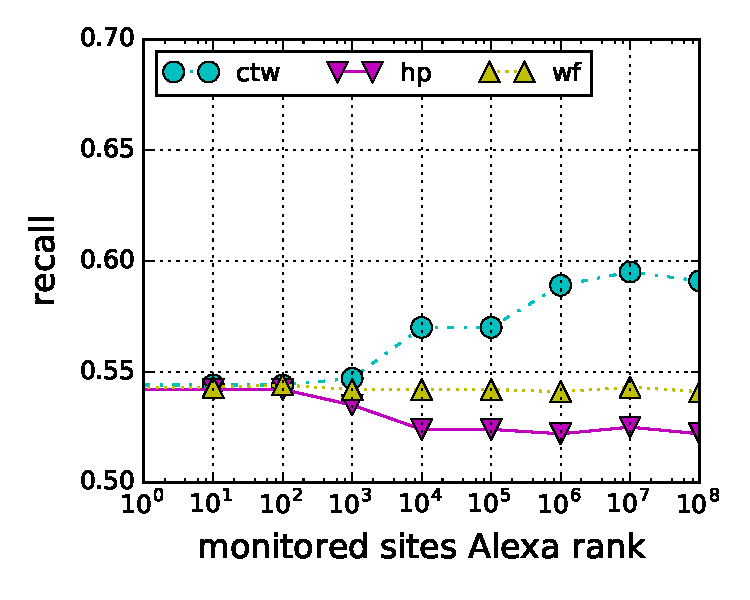
\includegraphics[width=0.466\linewidth]{figures/wfdns/alexa/1kx100+100k-offsets-100pct-recall}
    \label{fig:wfdns:alexa:recall}
}
\subfigure[Precision]{
	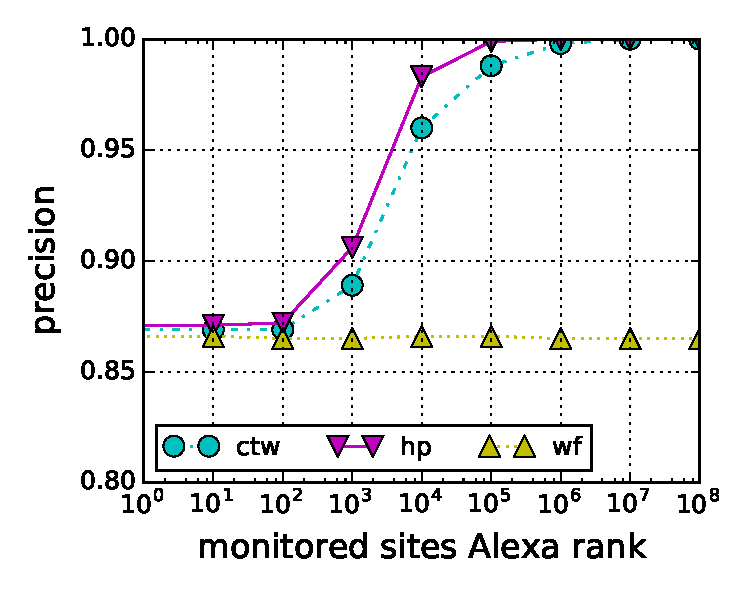
\includegraphics[width=0.466\linewidth]{figures/wfdns/alexa/1kx100+100k-offsets-100pct-precision}
    \label{fig:wfdns:alexa:precision}
}
\caption{The recall and precision when varying the starting Alexa rank of
monitored sites.}
\label{fig:wfdns:alexa}
\end{figure}

The above results paint a bleak picture: a small fraction of exit
bandwidth provides a perfectly precise attack on relatively
\emph{unpopular} sites such as \url{wikileaks.org} at Alexa rank 10,808.
To better understand the implications and limitations of our attacks,
from now on we focus on
33\% of exit bandwith (as observed on average by Google) and
precision (where we see clear gain from both our attacks).
Unless otherwise stated
we monitor pages starting from Alexa 10,000.

\begin{figure*}[t]
\centering
\subfigure[Approximating the impact of website fingerprinting defenses.]{
	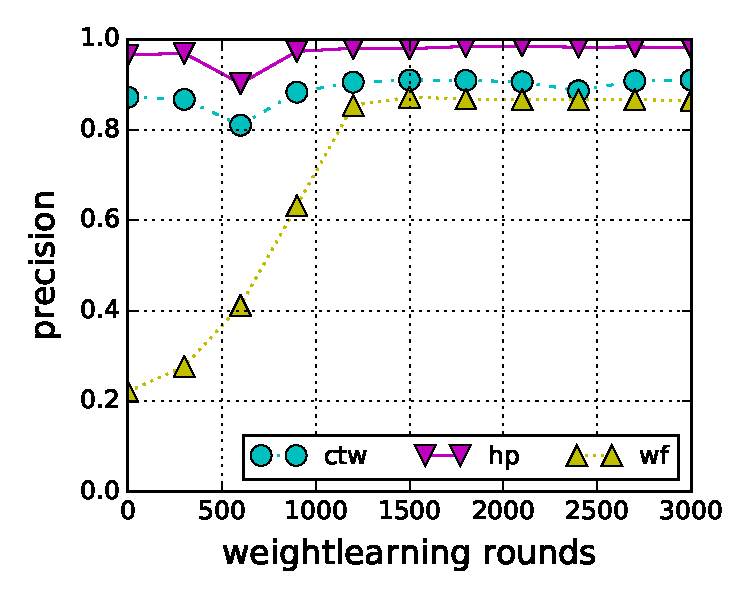
\includegraphics[width=0.23\linewidth]{figures/wfdns/rounds/1kx100+100k}
    \label{fig:wfdns:var:rounds}
}
\subfigure[Increasing the window size due to TTL clipping at Alexa 10k and 100k.]{
	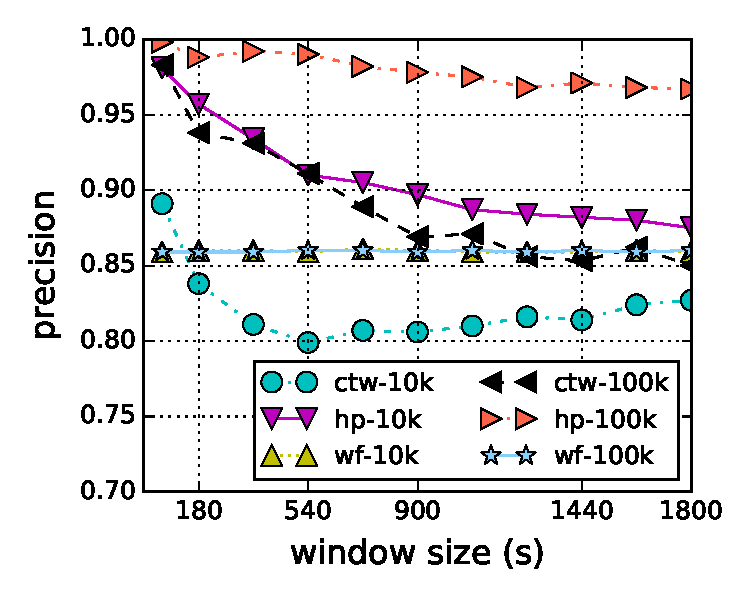
\includegraphics[width=0.23\linewidth]{figures/wfdns/window/1kx100+100k}
    \label{fig:wfdns:var:window}
}
\subfigure[Scaling the Tor network wrt. site visits at Alexa 10k and 100k.]{
	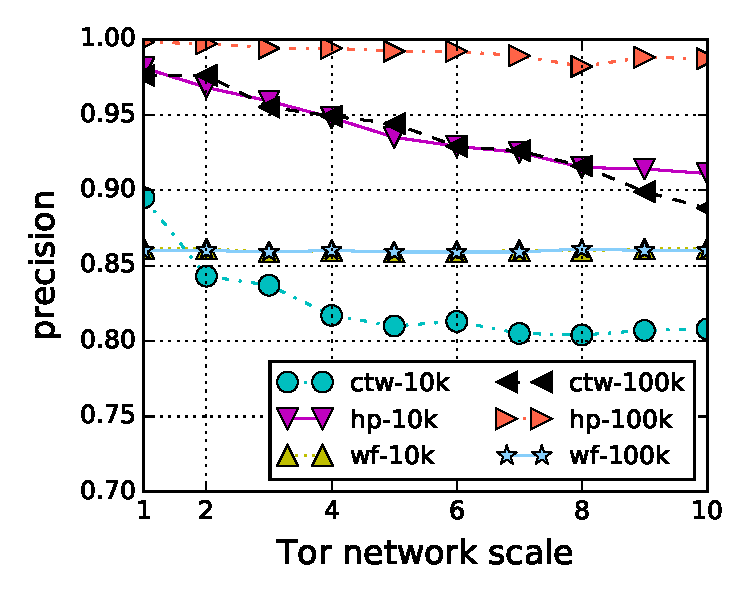
\includegraphics[width=0.23\linewidth]{figures/wfdns/scale/1kx100+100k}
    \label{fig:wfdns:var:scale}
}
\subfigure[The impact of different website popularity distributions.]{
	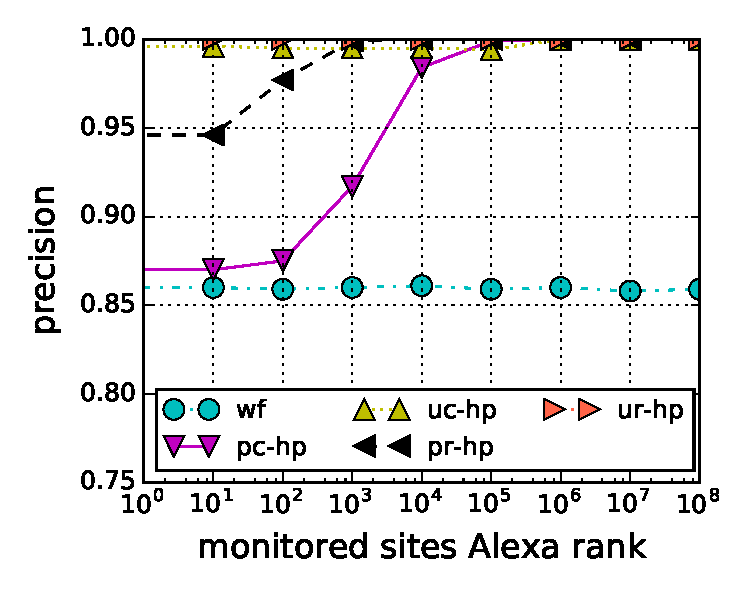
\includegraphics[width=0.23\linewidth]{figures/wfdns/dist/1kx100+100k}
    \label{fig:wfdns:var:dist}
}
\caption{The impact on the precision of our attacks when observing 33\% of Tor
exit traffic (Google's average). The defaults are: Alexa from top 10,000,
2500 weightlearning rounds,
60 seconds window size, Tor network scale 1.0, and the conservative
power-law distribution (pc) with $\alpha=1.13487087527372$.}
\label{fig:wfdns:var}
\end{figure*}



\subsection{Sensitivity to website popularity distribution}

% alexa offsets, all distributions and attacks
If we assume that our estimate for the number of sites visited through the Tor
network, as described in Section~\ref{sec:load-freq}, is roughly correct
(and we know from Figure~\ref{fig:wfdns:var:scale} that the effects of an error
is relatively minor) then one imporant consideration is how
these site visits are distributed. We define four distributions:
\begin{description}
	\item[pc] A conservative power-law distribution
	(with $\alpha=1.13487087527372$)
	that we manually fitted to the Alexa top 10,000 data,
	slightly underrepresenting the popularity of top Alexa sites.
	This distribution was described in Section~\ref{sec:attack:pop}.
	\item[pr] A realistic power-law distribution
	(with $\alpha=1.98331802607295$)
	that is the best fit according to
	the python power-law library by Alstott~\ea~\cite{power-law} for the Alexa
	top 10,000 data.
	\item[uc] A conservative uniformly random distribution that for some reason
	only considers one million active websites on the Internet.
	\item[ur] A realistic uniformly random distribution that considers 173 million active websites, as reported by Netcraft in July 2016.
\end{description}
Figure~\ref{fig:wfdns:var:dist} shows the effect on the precision of the
\texttt{hp} attack for the different distributions as we vary the starting
Alexa rank. The uniform distributions always have perfect precision.
The difference between the two power-law distributions is about one order of
magnitude in terms of starting Alexa rank: the realistic distribution gets
near perfect at 1,000 and the conservative at 10,000.
We conclude that WF+DNS attacks are perfectly precise for unpopular sites
where the probability that someone else than the target browses to a monitored
site within the timeframe given by the window length is negligible.


\subsection{Effect of website fingerprinting defenses}

Website fingerprinting defenses are being
designed and discussed for deployment in Tor.
The defenses produce bandwidth and/or latency overhead with a significant
increase in overhead the stronger the defense\footnote{e.g., Juarez et al.
observe an exponentially growing bandwidth overhead for increasing protection
with WTF-PAD~\cite{DBLP:journals/corr/JuarezIPDW15}.}.
This leads to the goal of finding an optima with ``good enough''
protection and minimal overhead.
As a first attempt to approximate the impact of fingerprinting
defenses on WF+DNS attacks, we use Wa-kNN with
random weights and no weightlearning: this significantly reduces the
effectiveness of the attack since some features (like indices of outgoing
packers) are several orders of magnitude more useful
than others~\cite{DBLP:journals/corr/JuarezIPDW15}.
Figure~\ref{fig:wfdns:var:rounds} shows the impact of doing between 0 and 3000
rounds of weightlearning. At few to no rounds precision for the \texttt{wf}
attack is below 50\%---the classification is more likely to be wrong than
right---while there is no impact on the \texttt{hp} attack and a relatively
small decrease for the \texttt{ctw} attack.
For recall (not shown in the figure), note the bound and relationship in
\ref{eq:hprecall}: for \texttt{wf} at 0 rounds the recall is 0.055 and for
\texttt{hp} 0.019. This suggests that for WF defenses to
be effective against WF+DNS attacks the defense must be tuned to provide a
low recall even when the parameters of WF attacks are selected for high
recall.

\subsection{Effect of Tor's TTL clipping}

\begin{table}[t]
\centering
\begin{tabular}{l r r}
\toprule
\textbf{TTLs} & \textbf{Median TTL (sec)} & \textbf{Mean TTL (sec)} \\
\midrule
% 2016/04/28 15:52:39 DNS records TTL mean 9780.0, std 42930.5, median 255.0, min 0.0, max 604800.0
raw & 255 & $9780.0\pm42930.5$ \\ % & 0 & 604800 \\
% 2016/04/28 15:44:05 DNS records TTL mean 701.5, std 755.3, median 255.0, min 60.0, max 1800.0
Tor & 255 & $701.5\pm\phantom{00}755.3$ \\ %& 60 & 1800 \\
% 2016/04/28 15:52:39 	unique domain TTL mean 13022.2, std 35054.4, median 900.0, min 0.0, max 604800.0
unique raw & 900 & $13022.2\pm35054.4$ \\ %& 0 & 604800 \\
% 2016/04/28 15:44:05 	unique domain TTL mean 1005.3, std 789.6, median 900.0, min 60.0, max 1800.0
unique Tor & 900 & $1005.3\pm\phantom{00}789.6$ \\ %& 60 & 1800 \\
% 2016/04/28 15:52:39 	unique domain _min_ TTL mean 3833.9, std 11073.6, median 60.0, min 0.0, max 604800.0
min unique raw & 60 & $3833.9\pm11073.6$ \\ % & 0 & 604800 \\
% 2016/04/28 15:44:05 	unique domain _min_ TTL mean 644.2, std 763.8, median 60.0, min 60.0, max 1800.0
min unique Tor & 60 & $644.2\pm\phantom{00}763.8$ \\ %& 60 & 1800 \\
\bottomrule
\end{tabular}
\caption{Mean and median DNS TTL values across Alexa top one million
  sites. Raw TTLs are unprocessed, as they appear in DNS lookup
  traces. Tor TTLs adhere to Tor's TTL clipping. 
Unique refers to the TTLs for unique domains; min unique only
considers the unique domains with the minimum TTL for each website.}
\label{tab:ttls}
\end{table}

As discussed in Section~\ref{sec:attack:sim}, due to a bug in Tor, the
maximum TTL for DNS responses in any Tor exit relay's DNS resolver cache
is 60 seconds. As a consequence, a sliding window of only the last 60
seconds of all observed DNS requests is enough to capture all visited
monitored sites through Tor (subject to the fraction of observed Tor
exit bandwidth, and mapping DNS requests to sites).

Table~\ref{tab:ttls} shows the TTL of DNS records in our dataset for the
TTL as-is (raw) and when clipped by Tor.  For each of these cases, we
also consider TTLs for all unique domains, and for only the unique
domain for each website with the lowest TTL.  About half of the sites on
Alexa top one million has a unique domain with a TTL of 60 seconds or
shorter; 48\% of the raw unique TTLs are below 60 seconds and only 26\%
above 30 minutes. Fixing the Tor clipping bug is therefore not
sufficient; to mitigate WF+DNS attacks, the minimum TTL should be 
significantly increased.  We also emulate what the correct TTL values
would be due to TTL clipping supposing that Tor eventually fixes the
aforementioned bug.  In this case, we find that Tor's TTL clipping has
no effect on the median TTL, but significantly reduces the mean TTL.

Suppose that Tor eventually fixes the DNS TTL bug, requiring the
attacker to monitor DNS lookups for a time interval equal to the maximum
TTL of all unique domains for any monitored site.
Figure~\ref{fig:wfdns:var:window} shows the effect on precision for
different time intervals from 60 seconds to 30 minutes (Tor's {\tt
  MAX\_DNS\_ENTRY\_AGE} for keeping entries in an exit's DNS resolver
cache) and for Alexa starting rank 10,000 and 100,000. For \texttt{ctw},
the time interval has a significant effect at both Alexa starting ranks,
while \texttt{hp} is only affected for sites ranked 100,000 or lower;
for more popular sites, the DNS lookup data still improves
fingerprinting precision, even with the larger window size.



\subsection{Effect of Tor network growth}
Figure~\ref{fig:wfdns:var:scale} scales the size of the Tor network with
respect to site
visits from the status quo to ten times its size, for Alexa starting rank 10,000 and
100,000. At twice its current size, the impact on WF+DNS attacks is smaller than
increasing the minumum TTL for DNS caching to 180 seconds as shown in
Figure~\ref{fig:wfdns:var:window}. These reulsts show that WF+DNS
attacks will remain
practical for unpopular sites, even as the network grows.

% limitation: webSITES, not wePAGES in our analysis + what we get from DNS.
